\chapter{Metodología y planificación}
\label{chap:Metodoloxía e planificación}
\lettrine{E}{n} esta sección se explica la metodología de trabajo empleada para el desarrollo del proyecto, así como la planificación del mismo.
Además, se describen los recursos utilizados y se hace una estimación de los costes asociados al proyecto.

\section{Metodología del desarrollo}
\label{sec:Metodoloxía do desenvolvemento}

Al ser un proyecto de investigación, la metodología de trabajo más adecuada es una metodología iterativa e incremental, que permite adaptarse a los cambios que van surgiendo durante el desarrollo del proyecto.
Esta metodología permite obtener un artefacto funcional al final de cada iteración, lo que permite obtener retroalimentación constante.
Cada iteración comienza con un análisis de lo que se quiere conseguir, seguida de las fases de diseño y codificación, y termina con una fase de testeo del producto.

\section{Planificación del proyecto}
\label{sec:Planificación do proxecto}
El proyecto inicialmente se divide en las siguientes fases principales:

\begin{itemize}
    \item \textbf{Revisión del estado del arte:}
    \begin{itemize}
        \item Estudio del dominio biológico: características de las imágenes oftalmológicas, su importancia y aplicaciones.
        \item Análisis de trabajos relacionados con IDIR, representaciones implícitas y segmentación de imágenes oftalmológicas mediante redes neuronales.
    \end{itemize}
    Esta fase se estimó en aproximadamente 3 semanas de trabajo, dada la necesidad de familiarizarse con el contexto e identificar soluciones previas relevantes.

    \item \textbf{Análisis del trabajo base:}
    \begin{itemize}
        \item Estudio en profundidad del código original de IDIR.
        \item Replicación de los resultados originales para verificar el funcionamiento correcto.
    \end{itemize}
    El esfuerzo estimado para esta tarea fue de 2 semanas, considerando el análisis del código y la puesta en marcha del entorno.

    \item \textbf{Adaptación al nuevo dominio:}
    \begin{itemize}
        \item Modificación de la arquitectura para trabajar con imágenes 2D en lugar de 4D.
        \item Implementación de las adaptaciones necesarias para imágenes oftalmológicas.
    \end{itemize}
    Esta etapa se estima una duración de 5 semanas, debido a la complejidad de las modificaciones y pruebas necesarias.

    \item \textbf{Evaluación y experimentación:}
    \begin{itemize}
        \item Diseño de una metodología de evaluación específica para el nuevo dominio.
        \item Realización de múltiples experimentos para optimizar el rendimiento.
        \item Validación de la efectividad en imágenes oftalmológicas.
    \end{itemize}
    Se estima un esfuerzo de 8 semanas, repartidas entre el diseño experimental, ejecución y análisis de los resultados de los distintos experimentos.

    \item \textbf{Documentación:}
    \begin{itemize}
        \item Redacción de la memoria final del proyecto.
        \item Análisis y presentación de los resultados obtenidos.
    \end{itemize}
    Para la documentación se reservaron 2 semanas, incluyendo la redacción, revisión y preparación de los anexos. La memoria será redactada a lo largo de todo el proceso, pero en esta fase final se revisará y completará.
\end{itemize}

En total, se estima una duración de 20 semanas para el proyecto, repartidas entre las distintas fases.
En la figura \ref{fig:planificacion_proxecto} se muestra el diagrama de Gantt que resume la planificación del proyecto, indicando las fases principales y su duración estimada.

\begin{figure}[tbp]
    \centering
    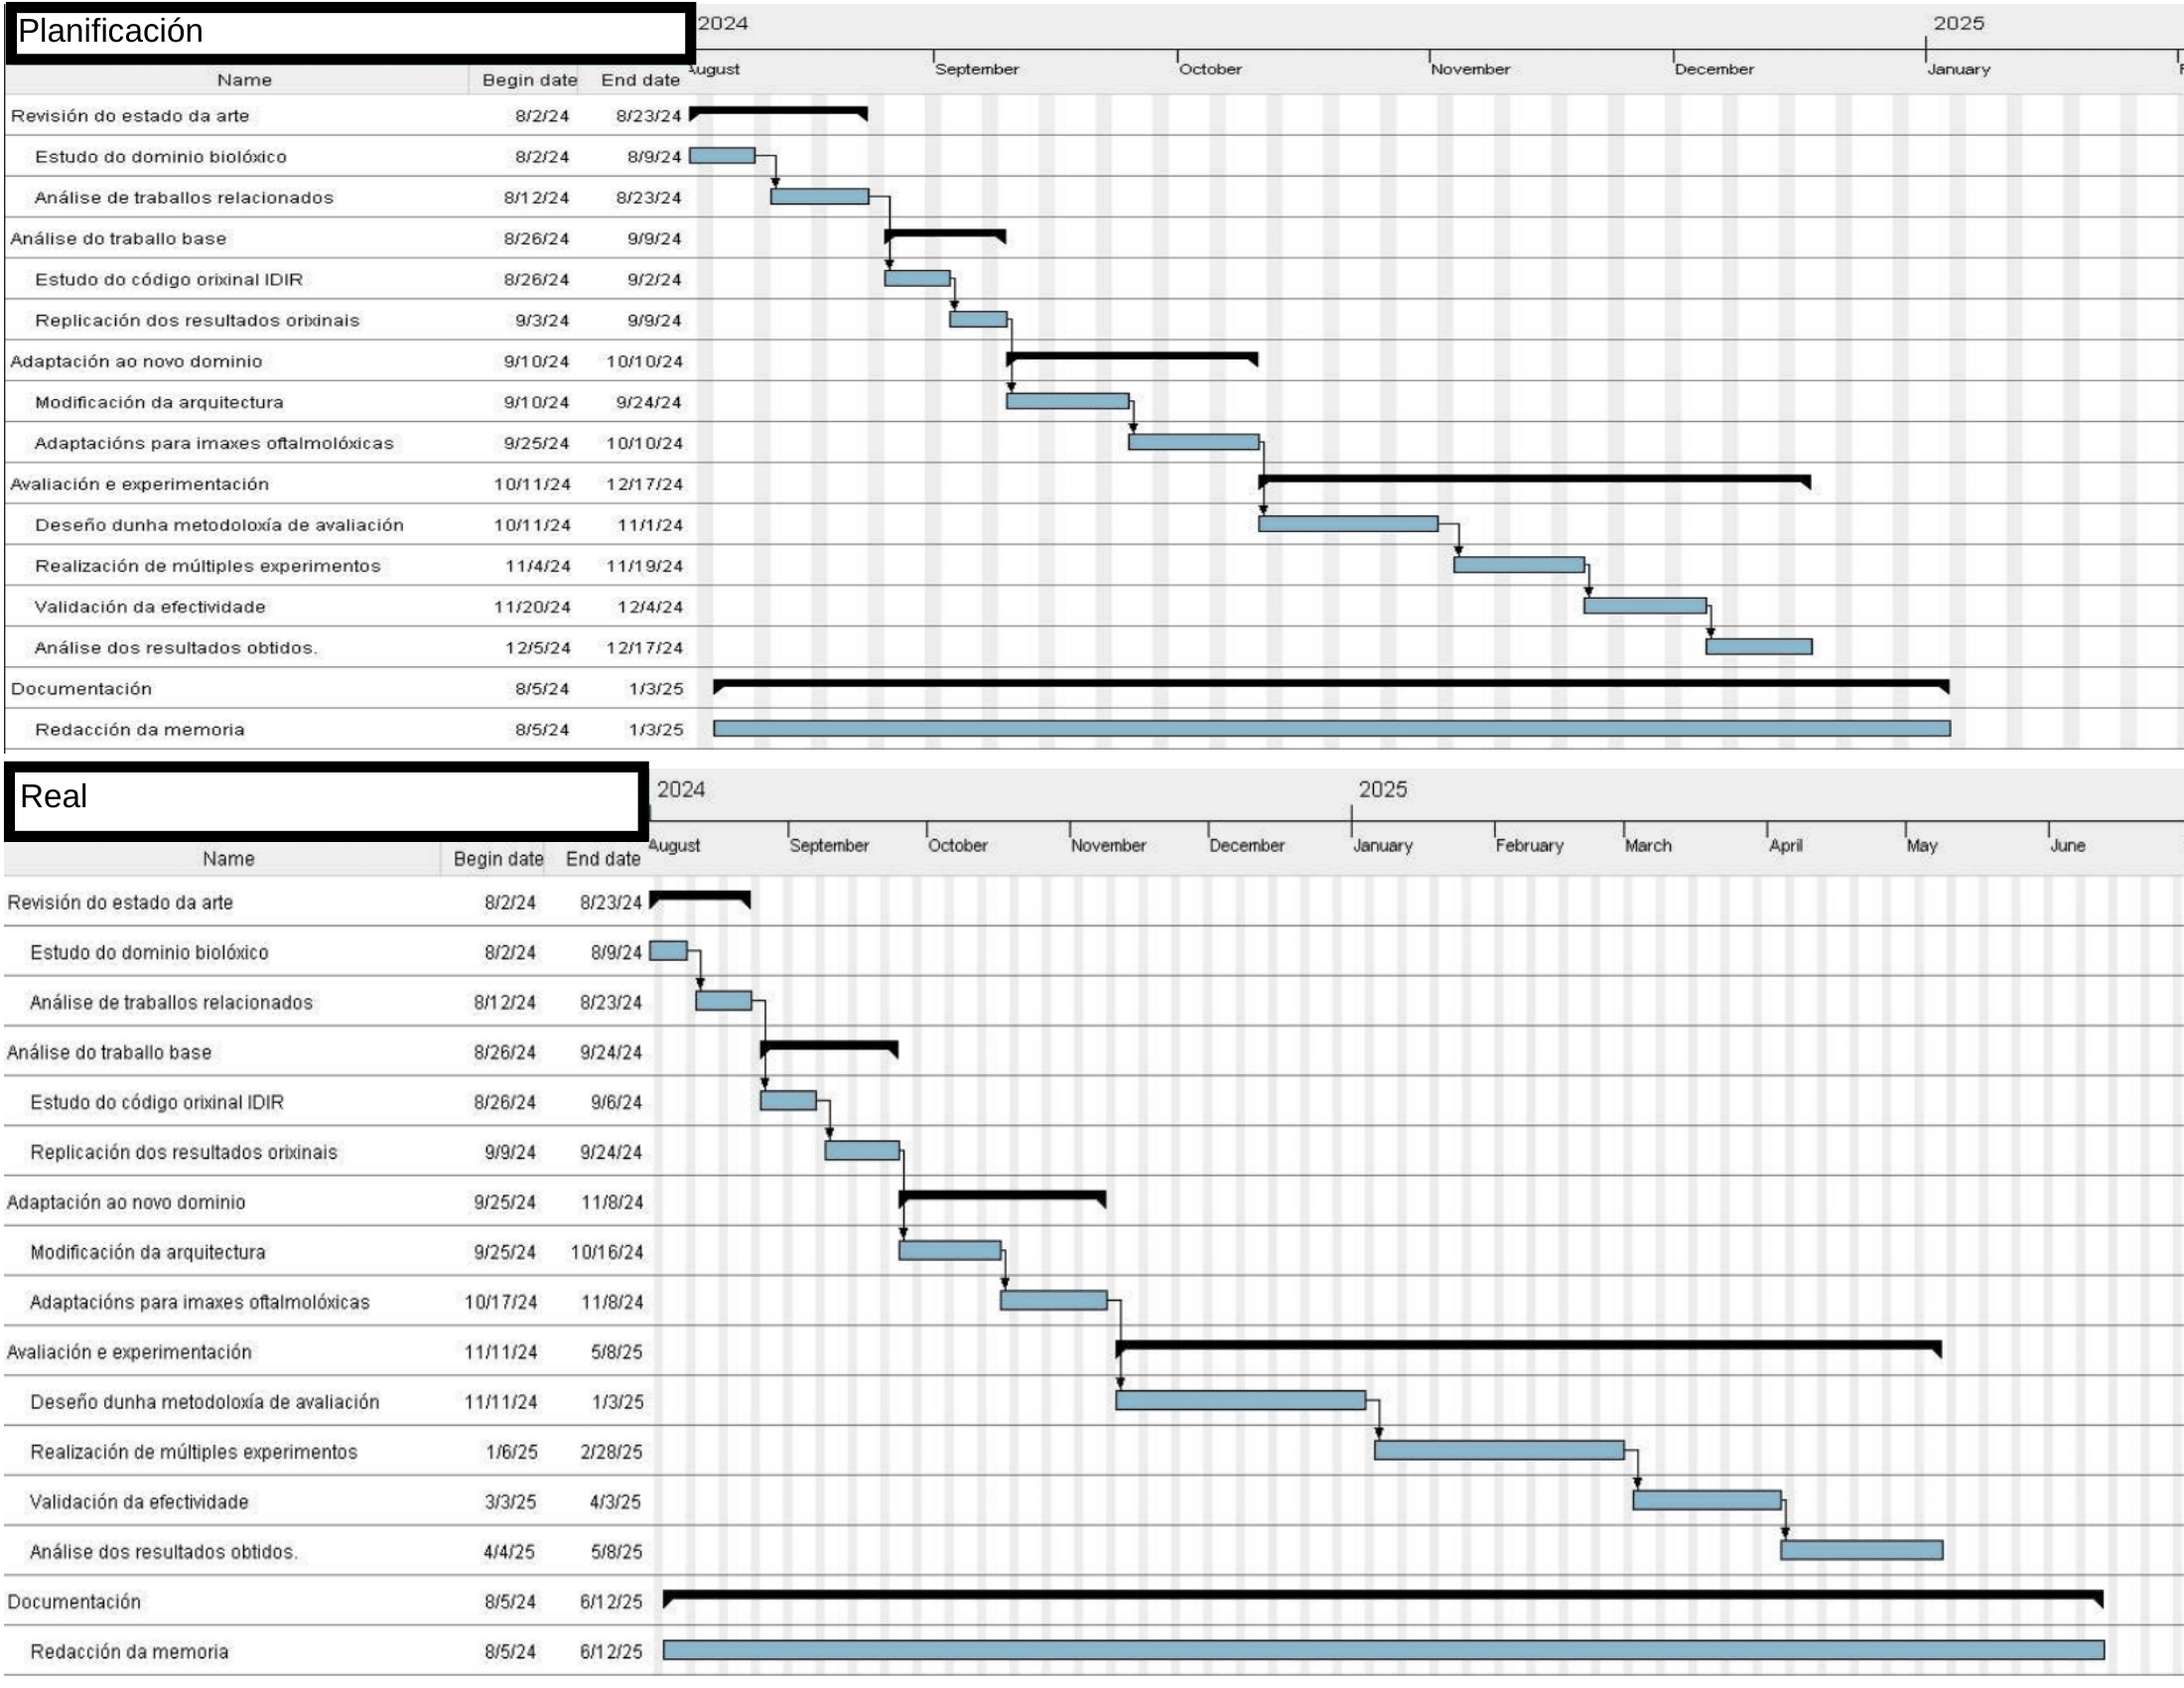
\includegraphics[height=1\textwidth, angle=90]{imaxes/gants-1.png}
    \caption{Diagramas de Gantt de la planificación del proyecto y duración real de cada fase}
    \label{fig:planificacion_proxecto}
\end{figure}

\section{Recursos utilizados}
\label{sec:Recursos utilizados}

\subsection{Software}
\label{subsec:Software}

Ya que parte del trabajo consiste en adaptar un trabajo previo,
se decidió emplear mucho del mismo software que el trabajo original para facilitar la implementación y reproducibilidad.
Lo más relevante es PyTorch, una librería de código abierto para Python que facilita la elaboración de redes neuronales. Se utilizaron las versiones de Python 3.12.3 y CUDA 12.2. También se emplean librerías de apoyo como NumPy (para trabajar con matrices), Matplotlib (visualización), OpenCV o scikit-learn (manejo de imágenes).

Otro software empleado incluye VSCode (IDE), Git (control de versiones) y LaTeX (redacción de memoria).

\subsection{Hardware}
\label{subsec:Hardware}

El proyecto fue desarrollado en un ordenador portátil conectado por ssh a un servidor con GPU.
Se utilizaron dos servidores diferentes, uno montado por mí\footnote{\url{https://blog.m19182.dev/writings/Building-my-Homelab}} y otro facilitado por el grupo de investigación VARPA (Visión Artificial y Reconocimiento de Patrones).

La gran parte de los experimentos fueron realizados en el primero, pero para poder ejecutar el proyecto con las imágenes en su resolución original fue necesario emplear el segundo
debido a las limitaciones de memoria de la GPU. En la tabla \ref{tab:comparativa_servidores} se muestra una comparativa entre los servidores utilizados, indicando las principales características de hardware de cada uno.

\begin{table}[tbp]
\centering
\begin{tabular}{|c|c|c|}
\hline
\textbf{Característica} & \textbf{Servidor Personal} & \textbf{Servidor VARPA} \\ \hline
Procesador & AMD Ryzen 9 5950X&  AMD Ryzen Threadripper 3960X \\ \hline
GPU & NVIDIA RTX 3090 & NVIDIA RTX A6000  \\ \hline
\end{tabular}
\caption{Comparativa entre los servidores utilizados}
\label{tab:comparativa_servidores}
\end{table}


\subsection{Conjuntos de datos}
\label{subsec:Conxuntos de datos}
Para el desarrollo del proyecto se emplearon dos conjuntos de datos diferentes:

\begin{itemize}
    \item \textbf{RFMID:} 3200 imágenes de fondo de ojo en color con resolución 1712x1712.
    \item \textbf{FIRE:} 134 pares de imágenes de retinas en color, con un tamaño de 2912×2912 píxeles
\end{itemize}

Estos son descritos en mayor detalle en la sección \ref{sec:Conxuntos de datos}.

\subsection{Estimación de costes}
\label{subsec:Estimación de custos}

Los costes del hardware son ignorados ya que ya estaba disponible antes de la realización del proyecto.

Los costes de los recursos humanos se calculan para un estudiante y dos tutores, resultando en un coste estimado de 20.680€, IVA incluido. La tabla \ref{tab:estimacion_custos} muestra la estimación de costes de los recursos humanos desglosados, considerando un estudiante a 20€/hora y tutores a 35€/hora.

\begin{table}[h]
\centering
\begin{tabular}{|c|c|c|c|}
\hline
\textbf{Recurso} & \textbf{Coste por hora} & \textbf{Horas estimadas} & \textbf{Coste total} \\ \hline
Estudiante & 20€ & 880h & 17.600€ \\ \hline
Tutor 1 & 35€ & 44h & 1.540€ \\ \hline
Tutor 2 & 35€ & 44h & 1.540€ \\ \hline
\end{tabular}
\caption{Estimación de costes de los recursos humanos (IVA incluido)}
\label{tab:estimacion_custos}
\end{table}

\section{Seguimiento de la planificación}
\label{sec:Seguimento da planificación}

La planificación del proyecto fue revisada periódicamente según las fases del proyecto, y para identificar desviaciones respecto al plan inicial.

A pesar de que en las fases iniciales del proyecto se respetó la planificación, la fase de adaptación al nuevo dominio y la fase de evaluación y experimentación sufrieron retrasos significativos.

La fase de adaptación al nuevo dominio requirió más tiempo del esperado debido a la complejidad de las modificaciones necesarias para adaptar el modelo a imágenes 2D, así como a la necesidad de realizar múltiples pruebas para garantizar el correcto funcionamiento del modelo adaptado. La fase de evaluación también se vio afectada, ya que requirió más tiempo del esperado para diseñar una metodología de evaluación adecuada. Finalmente, la fase de experimentación requirió más tiempo del previsto, en parte debido a los malos resultados obtenidos inicialmente, que obligaron a revisar en profundidad el código e implementar nuevas pruebas para asegurar la correcta implementación.
En total, esto conllevó un retraso de aproximadamente 18 semanas respecto a la planificación inicial.

La fase final de análisis de resultados y redacción de la memoria también se vio afectada, aunque en menor medida, lo que conllevó un retraso adicional de 2 semanas, resultando en una duración total del proyecto de 40 semanas, frente a las 20 semanas inicialmente previstas.

En la figura \ref{fig:planificacion_proxecto} se muestra el diagrama de Gantt actualizado, que refleja la duración real de cada fase del proyecto.

\subsection{Estimación de coste real}
\label{subsec:Estimación de custo real}

La estimación de coste del proyecto fue de 20.680€, como se indicó en la sección \ref{subsec:Estimación de custos}. No obstante, debido a los retrasos en el desarrollo del proyecto, el coste real aumentó de forma proporcional al tiempo extra empleado.

Dado que el proyecto se extendió durante 20 semanas más de lo previsto (el doble de la planificación inicial), el coste real estimado asciende a 41.360€ (IVA incluido).